% Communication lessons I take from open-ended fields: we should say GCP will *stop* CC (not limit it under 2°C, because people still feel that it only reduces the problem but doesn't solve it), and that it will cost nothing to typical people (i.e. tie it to national redistribution)
% TODO! add that govts would raise taxes following the gbi
% TODO! change from 2°C to 1.5 °C (cf. email Climate Analytics)
% TODO! Article 6-4 of the Paris agreement stipulates that a fraction (5% according to South Africa gov though the agreement doesn't specify a figure) of global carbon market revenues should finance adaptation
% TODO! question of forest, low-carbon finance, 
\documentclass[12pt,english]{article}
\usepackage[utf8]{inputenc}
\usepackage{tgpagella} % Palatino text only
\usepackage{mathpazo}  % Palatino math & text
\usepackage[left=1.5in,right=1.5in,top=1.5in,bottom=1.5in]{geometry}
% \linespread{1.5}
% \usepackage[super,comma,sort]{natbib}
\usepackage[round,sort&compress]{natbib}
\usepackage{url} % [hyphens]
\usepackage[hyperpageref]{backref} % back references biblio. Needs latexmk at compilation.
\usepackage[pagebackref]{hyperref}
% \usepackage{multibib} % incompatible with backref
\hypersetup{
  colorlinks=true, % breaklinks=true,
  urlcolor=purple,    % color of external links
  linkcolor=blue,  % color of toc, list of figs etc.
  citecolor=violet,   % color of links to bibliography
}
\usepackage{bm}
\usepackage{indentfirst}
\usepackage{tocbibind}
\setcitestyle{aysep={}} 
\usepackage{amsmath}
\usepackage{amssymb}
\usepackage{eurosym}
\usepackage{amsfonts}
\usepackage{enumerate}
\usepackage{babel}
\usepackage{caption}
\usepackage{supertabular}
\usepackage{tabularx}
\usepackage{float}
\usepackage{dsfont}
\usepackage{fancyvrb}
\usepackage{verbatim}
\usepackage{enumitem}
\usepackage{setspace}
\usepackage{comment}
\usepackage{subcaption}
\usepackage{graphicx}
\usepackage{tikz}
\usepackage{gensymb}
\usepackage{textcomp}

\usepackage{tabulary}
\usepackage{tabularx}
\usepackage{booktabs}
\usepackage{fullpage}
\usepackage{morefloats}
\usepackage{makecell}
\usepackage{lscape}
\usepackage{pdflscape}
\usepackage{longtable}
\usepackage{rotating}
\usepackage{xcolor}% header
\usepackage{titlesec} % To change size of Bibliography heading
\usepackage{fancyhdr}

% Header on every page except frontpage (handled by tikz)
% \pagestyle{fancy}% header
% \renewcommand{\headrulewidth}{0pt} % removes horizontal line from header
% \setlength{\headheight}{62pt} % adjust the nb of pt here and below if there is a warning
% \addtolength{\topmargin}{-62pt}
% \fancyhead[R]{} % removes section title from header
% \fancyhead[L]{} % removes section title from header
% \chead{\href{http://global-redistribution-advocates.org}{
\includegraphics[height=1cm]{../figures/policies/logo_full_white_bg}}\\ \quad }

\usepackage{tocloft}
\usepackage{titletoc}
\usepackage{csquotes}
\usepackage{tcolorbox}
\usepackage[export]{adjustbox}
\usepackage[anythingbreaks]{breakurl} % for links
\usepackage{multicol}
\newsavebox\ltmcbox % For net gain table over two columns
%\usepackage[nomarkers,figuresonly]{endfloat} % Figures at the end
%\usepackage[section,below]{placeins} % Floats placed in the section they appear in.
\renewcommand{\floatpagefraction}{.9}

\title{The Global Climate Plan -- Policy Brief
} 

\author{\textcolor{white}{Adrien Fabre\footnote{\textcolor{black}{The author is Adrien Fabre, CNRS researcher in economics at CIRED. E-mail: adrien.fabre@cnrs.fr.}}}
%\footnote{CNRS researcher in economics at CIRED. E-mail: adrien.fabre@cnrs.fr.}
} 
% \author{Global Redistribution Advocates\footnote{The author is Adrien Fabre, CNRS researcher in economics at CIRED. E-mail: adrien.fabre@cnrs.fr.}} 

\date{\today{} -- \href{https://github.com/bixiou/global_tax_attitudes/raw/main/paper/policy_brief_GCS.pdf}{Link to most recent version}} 

\begin{document}

\maketitle
\tikz [remember picture, overlay] %
\node [shift={(5.5cm,-1.5cm)}] at (current page.north west) % north west
[anchor=north west] % north west
{\href{http://global-redistribution-advocates.org}{
\includegraphics[height=1.3cm]{../figures/policies/logo_full_white_bg}}};

% \begin{center}
% {\textbf{\href{https://github.com/bixiou/global_tax_attitudes/raw/main/paper/policy_brief_GCP.pdf}{Link to most recent version}}}
% \end{center}

% Summary: survey description + results
% Principle. Link to econ theory, CBAM/carbon market merge, SDGs.
% Distributive effects.
% Acceptation
% Details of the agreement
% Details of implementation (e.g. Aadhaar)
% TODO! add possibility to tax + necessity to fund infra/public services
% TODO! cite Feasta (done) / CapGlobalCarbon / Sharing for survival (enquiring technos required to distribute cash)
% TODO! basic income or (unconditional) cash transfer?
% TODO? add interdiction of yachts and private jets?

% TODO? switch to stable/perpetual basic income? Present results of costs/transfers in terms of NPV? (e.g. the GCP would raise 2.2% of GDP in NPV)
% I am amazed in that the stable basic income is not so reduced compared to the basic income at its peak/plateau (~$50/month). With an interest rate of 4%, I find a stable BI of $39, and with r = 2% => BI = $28. It seems indeed a good idea to provide a stable basic income, especially if it can be only 20% lower than the inverse-U shaped one at its peak. 
% But practical questions arise: How to choose the interest rate? Who can be the intermediary and provide the maturity transformation? Is there a market for perpetual bonds? Should the governments set up a dedicated financial institution?

\section{Summary}\label{sec:intro}

\begin{quote}
  ``At the Paris agreement in 2015, all countries have agreed to contain global warming `well below +2 $\mathrm{{}^\circ}$C'. To limit global warming to this level,~\textbf{there is a maximum amount of greenhouse gases we can emit globally}.\\
  To meet the climate target, a limited number of permits to emit greenhouse gases can be created globally. % TODO? CO2 instead of GHG?
  Polluting firms would be required to buy permits to cover their emissions. Such a policy would~\textbf{make fossil fuel companies pay}~for their emissions and progressively raise the price of fossil fuels.~\textbf{Higher prices would encourage people and companies to use less fossil fuels, reducing greenhouse gas emissions.}\\
  In accordance with the principle that each human has an equal right to pollute, the revenues generated by the sale of permits could finance a global basic income.~\textbf{Each adult in the world would receive } \$30/month, thereby lifting out of extreme poverty the 700 million people who earn less than \$2/day.\\
  \textbf{The typical }[\textbf{American}]\textbf{ would lose out financially }[\textbf{\$85}]\textbf{ per month}~(as he or she would face [\$115] per month in price increases, which is higher than the \$30 they would receive).\\
  The policy could be put in place as soon as countries totaling more than 60\% of global emissions agree on it. Countries that would refuse to take part in the policy could face sanctions (like tariffs) from the rest of the World and would be excluded from the basic income.''
\end{quote}

In a representative survey on 3,000 respondents, \citet{fabre_international_2023} show that 54\% of Americans support the Global Climate Plan (GCP) as described above. Actually, \citet{fabre_international_2023} also run the survey on 3,000 Europeans (representative of France, Germany, Spain and the UK) and find that 76\% of them support the GCP. Moreover, they report results of a survey on 40,680 respondents in 20 countries covering 72\% of global CO$_\text{2}$ emissions which finds strong majority support in each country for such a policy.% , \citet{dechezlepretre_fighting_2022}

In this policy brief, we make the case for a Global Climate Plan. We show that it is grounded on solid ethics and economics (Section \ref{sec:principles}), would operate a global redistribution from rich to poor (Section \ref{sec:distribution}), can be implemented with current technology (Section \ref{sec:implementation}), and is genuinely supported by the population across the World (Section \ref{sec:support}). Finally, we expand on the above description and formulate a well-specified plan (Section \ref{sec:details}).

\section{Principles}\label{sec:principles}
% Paris agreement, SDGs
The Global Climate Plan would help achieving the internationally agreed agenda for a prosperous future. While the Paris agreement sets an unanimous climate objective, it does not establish binding rules, and current policies place the world on track to a temperature rise of 2.7\textdegree{}C in 2100 \citep{climate_action_tracker_warming_2022}. Likewise, the Sustainable Development Goals set different targets for 2030, the first one being to eradicate extreme poverty defined as living on less than \$1.90 a day (in 2011 PPP). % TODO? \$2.15 a day (in 2017 PPP)
We are not on track to achieve this target, as 8\% of the world population still live in extreme poverty \citep{un_sustainable_2022}. Meanwhile, the nominal GDP per capita (in 2021) is \href{https://data.worldbank.org/indicator/NY.GDP.PCAP.CD?end=2021&locations=EU-ZG-XD-XM-1W-IN-US-CD-BI-LU-CN&start=2021&view=bar}{62 times larger} in high-income countries (home to 1.2 billion people) than in low-income countries (700 million), meaning that a transfer of just 1\% of high-income countries' GDP would mechanically double low-income countries' national income. 

By design, the Global Climate Plan (GCP) would stop global warming at a reasonable level, eradicate extreme poverty, and make a dent on global inequalities. It builds on the cap-and-share proposals by \citet{grubb_greenhouse_1990}; \citet{feasta_cap_2008} and relies on four principles:

\paragraph*{1. A cap on emissions to meet the 2\textdegree{}C target.} 

%To limit global warming to 2\textdegree{}C with 67\% probability, we can deduce from the \citet{ipcc_climate_2021} and \href{https://ourworldindata.org/co2-emissions#global-co2-emissions-from-fossil-fuels-and-land-use-change}{current emissions} that the world has a remaining carbon budget of about 1,000GtCO$_\text{2}$ starting from 2024. 
% computed using 37.5G/year https://ourworldindata.org/co2-emissions#global-co2-emissions-from-fossil-fuels-and-land-use-change and IPCC SPM.2
The \citet{ipcc_climate_2021} provides the carbon budget that remains to limit global warming to ``well below 2\textdegree{}C''. 
Defining a global emissions trajectory and imposing a yearly quota on global CO$_\text{2}$ emissions would ensure that they decrease in line with the target. 
Emissions permits corresponding to the quota would then be auctioned ``upstream'' to industrial units that emit CO$_\text{2}$ or sell fossil fuels (like refineries, coal mines, or cement plants). 
% Trading of emissions allowances allows to reach efficiency in emissions reductions. 
In short, an Emissions Trading System (ETS) would be established to control CO$_\text{2}$ emissions at the global level. 
Implemented in various countries including the European Union, China, and South Korea, and being under consideration in others like India, Brazil or Nigeria, ETSs already cover 17\% of global GHG emissions. They can be successfully linked to one another, as California and Québec showed \citep{icap_emissions_2023}. 
% the EU, China, California, South Korea, Québec, Mexico, (Kazakhstan)

\paragraph*{2. Defending the interests of people rather than nations.}
Although global carbon pricing has long been discussed, it has stumbled upon the allocation of emissions entitlements between countries. 
For example, the U.S. has historically defended the free allocation of emissions permits to emitting sources while India has insisted on the historical responsibility of industrialized countries to defend a redistributive solution \citep{bertram_tradeable_1992,michaelowa_report_2012}. 
An approach centered on individuals rather than countries helps escaping this impasse. Indeed, as shown in Section \ref{sec:support}, there is a worldwide consensus in favor of an equal right to emit for each human. 
Compared to other approaches, the egalitarian allocation has the merit of simplicity and provides a clear focal point. 
What is more, the individual approach can also be applied to address historical responsibilities, by redistributing individual wealth rather than attributing climate debts to industrialized countries. In a \href{https://github.com/bixiou/global_tax_attitudes/blob/main/paper/policy_brief_tax.pdf}{separate policy brief}, % TODO update link
we propose a global wealth tax that would finance low-income countries as well as carbon removal. 
%To showcase the individual approach, it is worth introducing a thought experiment. Imagine if, in year 2000, all capital owners voluntarily redistributed their assets so that each human would get an equal wealth. In this utopian world, all countries now enjoy similar standards of living. Would it still make sense to transfer resources from the U.S. to India on the ground of historical responsibilities? Would it make sense to transfer resources from one person who gave away all their wealth to another person, now richer than the first, because the first one polluted more in the past?
Indeed, the best available approximation of the historical emissions of someone is arguably their wealth or, if the person died, the wealth of their descendants. Besides, ability to pay of individuals may be better suited than past emissions of countries to define fair shares of the decarbonization burden. % For example, should a person enjoy a lesser burden if they choose to live in France rather than Germany, on the ground that France historically decided to replace coal by nuclear in its electricity mix?
% Because carbon emissions were parallel to capital accumulation, countries that emitted more in the past tend to be richer today. But this is not always true (think of Ukraine). We argue that
% Past emissions disproportionally benefitted wealthy people, as carbon footprint increases with wealth. Attributing historical responsibilities to wealthy people

The GCP is a good complement (rather than a substitute) to other climate or redistributive policies \citep{stiglitz_addressing_2019}. In particular, the GCP's negative effect on the purchasing power of an average emitter of a high-income country can be offset by national redistribution, through increased income taxes on the top 5\%. Furthermore, some decarbonization costs can be mutualized, e.g. through public investments in public transportation and subsidies to thermal insulation, to reduce the discrepancy in private costs between people with similar income but different carbon footprint. The GCP actually encourages complementary decarbonization policies, as countries decarbonizing faster will contribute less to the GCP revenues than countries entirely relying on the price mechanism. %Finally, financial actions are needed to de-risk low carbon projects (especially in low-income countries) and unleash green investments (\href{https://www.foreign.gov.bb/the-2022-barbados-agenda/}{Bridgetown Initiative}, \citealp{hourcade_accelerating_2021}). %which reduce the reliance on the carbon price incentive to decarbonize, 
% equal right to emit; efficiency of pricing, simplicity of rights allocation, complementarity with other climate & redistributive measures
% TODO put last sentence in position paper (or put back here?)

\paragraph*{3. A global basic income that eradicates extreme poverty.}

The GCP revenues would be used to finance a global basic income. At their peak, assuming a carbon price of \$150/tCO$_\text{2}$ in 2030, the GCP revenues are estimated to amount to 5\% of the Gross World Product. The GCP would entail 0.9\% of the GWP in net international transfers -- the major part being disbursed in the country it is collected (see Section \ref{sec:distribution}). %At their peak,  assuming a carbon price of \$90/tCO$_\text{2}$ in 2030, the GCP revenues are estimated to amount to 1.7\% of the Gross World Product, including 0.7\% in international transfers (see Section \ref{sec:distribution}). 
Using a scenario limiting global warming to 1.8\textdegree{}C,%\footnote{We use the emissions trajectory from the Efficiency scenario (2\textdegree{}C with $>$50\% chance) of the Global Energy Assessment \citep{johansson_global_2012} and the price trajectory of SSP2-2.6 \citep{fricko_marker_2017}. See details in \citet{fabre_international_2023} and the code on \href{https://github.com/bixiou/global_tax_attitudes/blob/main/code_global/map_GCP_incidence.R}{github}.} %report by \citet{stern_report_2017} 
we estimate that the basic income would amount to \$47 per month for each human above 15 in 2030, enough to lift out of extreme poverty the 700 million people who live with less than \$2.15 a day. % TODO: specify how % TODO! which carbon budget is that?
Conversely, high emitters like a typical British person (with median British CO$_\text{2}$ emissions) would lose in net \$23 per month, as they would face \$70 per month in price increases. %Overall, the GCP would operate substantial international transfers, estimated in Section \ref{sec:distribution}.  
Although the GCP revenues will fall when decarbonization nears completion (around the 2060s), the global basic income should be sustained using new sources of funding (e.g. a global corporate tax). 

Although distributing a basic income to every human is technically challenging, different options are available, reviewed in Section \ref{sec:implementation}. 

\paragraph*{4. A climate club to foster global cooperation.}

Building on insights from game theory \citep{mackay_price_2015, nordhaus_climate_2015}, the GCP should be launched by a club of willing countries, with carbon border adjustments and possibly sanctions on non-participating countries, to foster compliance by most countries. 
The GCP would be implemented as soon as 60\% of global CO$_\text{2}$ emissions are covered by the parties. This threshold can be met by the union of China (30\% of global emissions), the U.S. (15\%), India (7\%), the EU and the UK (9\%); or, if the U.S. do not participate,\footnote{Note that some U.S. States could still participate even if the federal level does not.} by the EU, the countries that would gain from the GCP (23\%, including India), and those that would neither gain nor lose (35\%, including China).

% 
% high CBAM for non-participants + possibly other sanctions (like on travel)
% USA: 15, In: 7, CN: 30, EU: 9, gain >0: 21 (gain >0 wo In: 14)
% a cap on emissions to meet the 2°C target
% granting an equal right to emit to each human / defending interests of people rather than nations
% a global basic income that eradicates extreme poverty
% a climate club (or sustainable union) to foster global cooperation

%Postulating %Assuming
% that each human has an equal right to emit CO$_\text{2}$, low emitters have a legitimate claim \textit{vis-à-vis} high emitters, that can be settled by monetary transfers. Coupling this burden-sharing principle to the carbon budget (remaining emissions that would be compatible with the Paris agreement) naturally defines a global climate policy. We call it the ``Global climate Plan'' (GCP); it consists of a global cap-and-trade system where emission rights are auctioned each year to polluting firms and the revenues finance a global basic income. 


\section{Distributive effects}\label{sec:distribution}

The GCP would redistribute income from high-emitters (people with a carbon footprint higher than the world average) to low-emitters. Indeed, polluting firms would pass on the carbon price to consumers, who will ultimately pay higher costs in proportion to their carbon footprint. The basic income amounts to the global average revenues per capita and would thus equal the carbon price times the global average carbon footprint. 

Currently, countries' footprints are strongly correlated (at .69) with their GDP per capita. But certain countries, like China, Iraq, or South Africa, have a carbon footprint higher than predicted by their GDP per capita. Section \ref{sec:details} describes an opt-out provision allowing these countries to participate in the carbon pricing without mutualizing the revenues. In addition, it might be the case that around 2050, countries like the EU will reach very low carbon footprint, perhaps lower than some developing countries like India. EU's footprint is currently 4 times higher than India's, so it would take time before a reversal can happen between the two. Still, Section \ref{sec:details} proposes a solution to prevent the GCP from redistributing from lower income to higher income countries.

\begin{figure}[h!]
    \caption{Estimated trajectories of emissions, carbon price and (adjusted) basic income.}\label{fig:trajectory}
    \makebox[\textwidth][c]{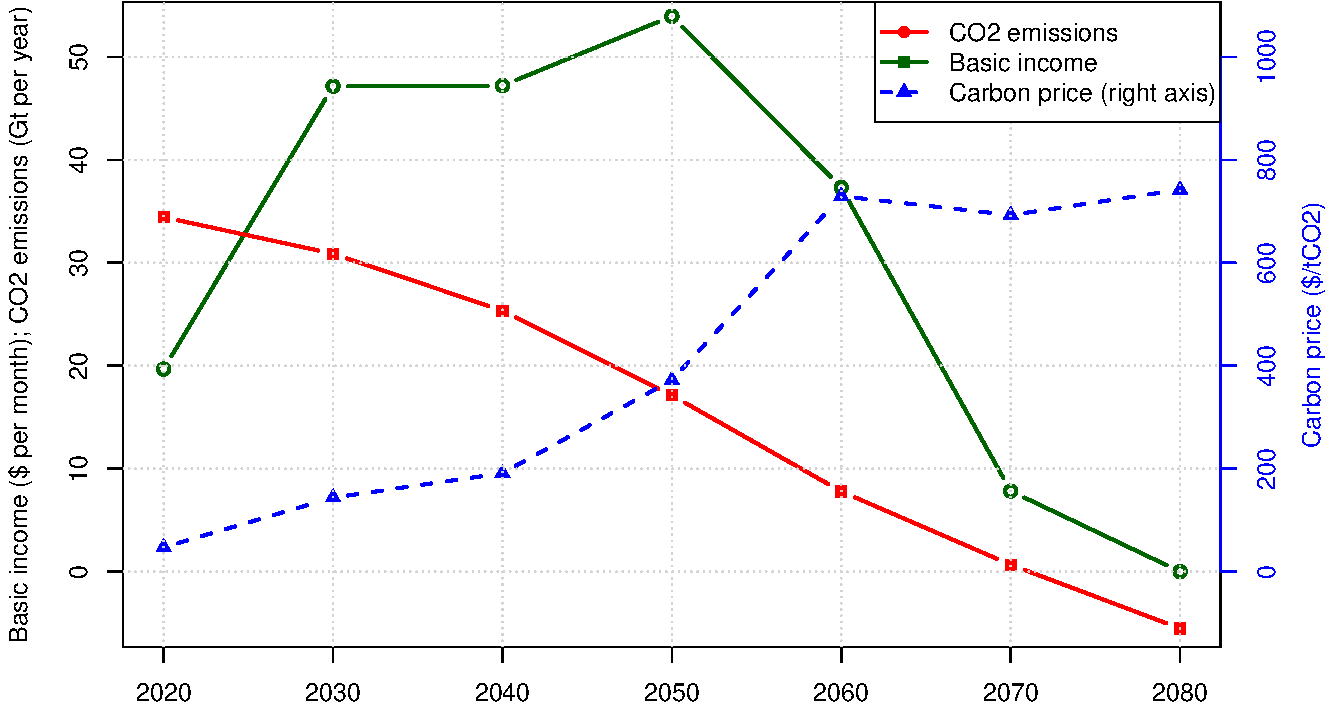
\includegraphics[width=.8\textwidth]{../figures/policies/GCS_adj_trajectories.pdf}} 
\end{figure}

\begin{figure}[h!]
    \caption{Net gains in 2030 from the Global Climate Plan with full participation.}\label{fig:median_gain_2015}
    \makebox[\textwidth][c]{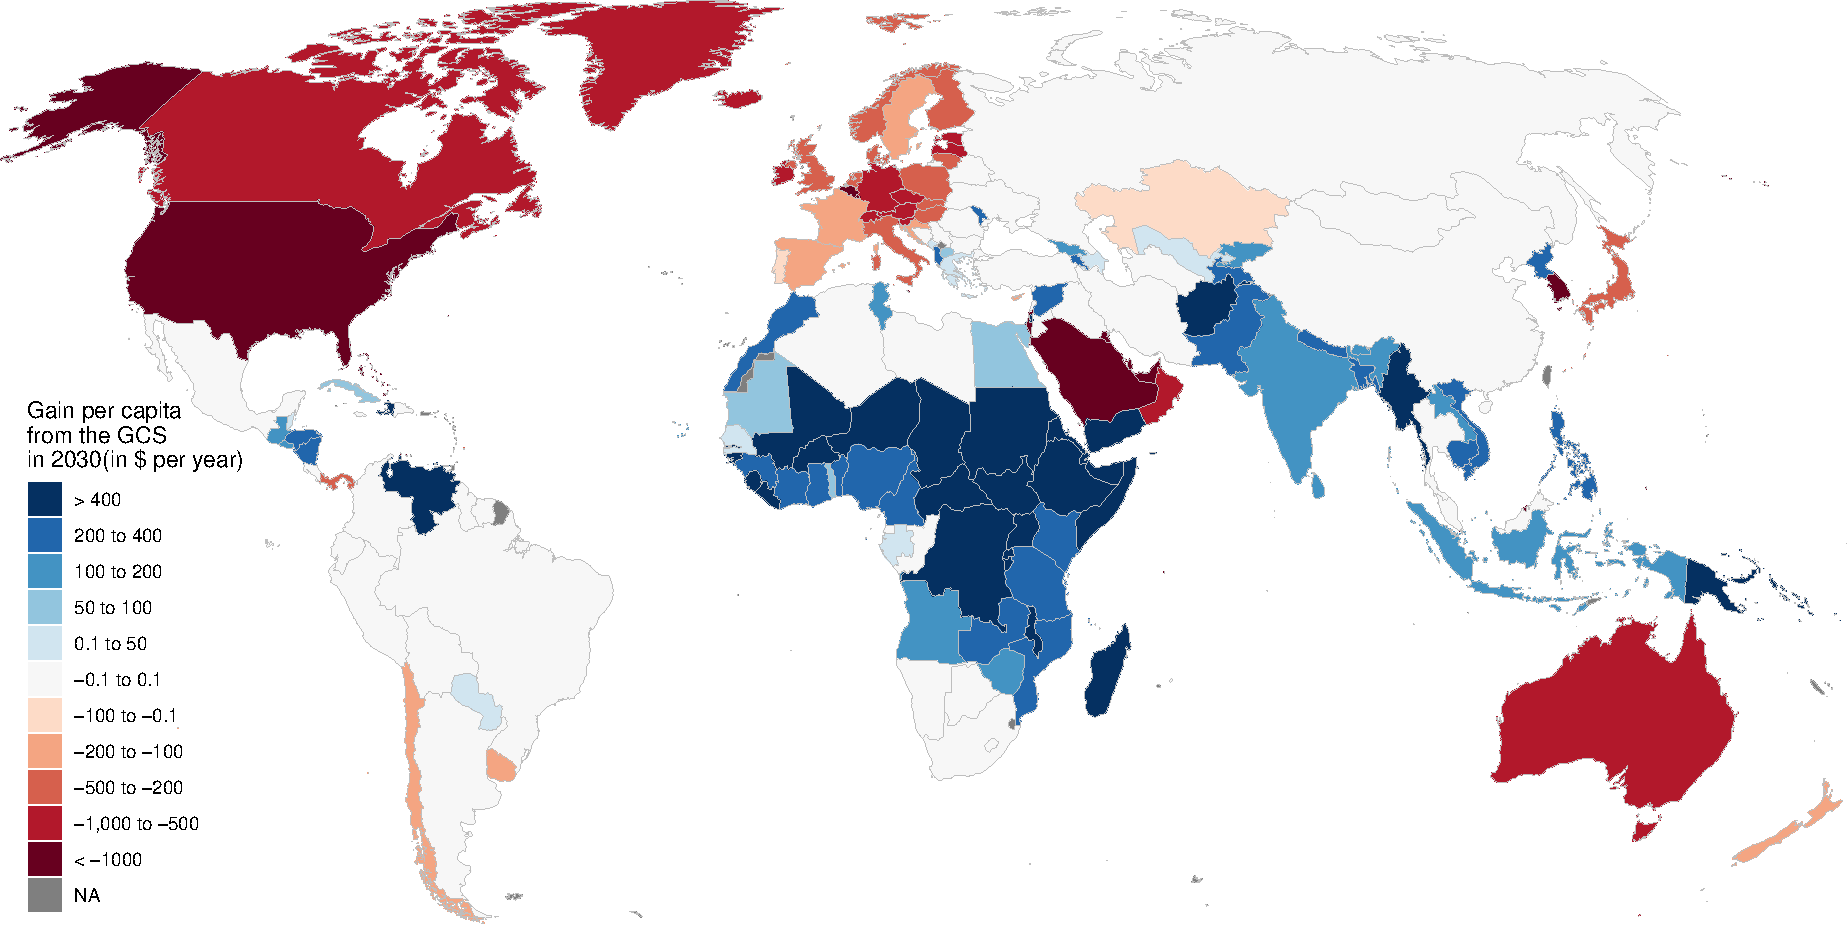
\includegraphics[width=\textwidth]{../figures/maps/gain_adj_2030.pdf}} % mean_gain_over_gdp_2019 mean_gain_2030
\end{figure}

\begin{tcolorbox}
  {\small
  \paragraph{How we compute the distributive effects}
  To specify the GCP, we use the Efficiency scenario of the Global Energy Assessment (GEA) by \citet{johansson_global_2012}, which gives a global CO$_\text{2}$ emissions trajectory consistent with limiting the global average temperature increase to 2\textdegree{}C with a probability of at least 50\%. We use the price trajectory of scenario SSP2-2.6 \citep{fricko_marker_2017} compatible with this emissions trajectory. 
  The product of these two series provides an estimate of the revenues expected from a global carbon price. We then divide it by projections (computed from the total population of the GEA and the UN median demographic scenario) of population over 15 years of age (\textit{adults}, for short) to derive the unadjusted basic income.  

  GEA provides emissions and GDP trajectories for 11 macro-regions. To estimate the increase in fossil fuel expenditures per adult (or ``cost'') and GDP per capita in each country, we make a key assumption concerning their evolution: that they will evolve by the same factor in each country of a same macro-region. To avoid a blatant violation of this assumption in the case of Botswana, Equatorial Guinea, Gabon, Namibia, and South Africa (whose GDP per capita was supposed to grow from 30\% to 200\% of the world average in 50 years), we attached them to the Middle-East--North Africa region (which is closer in terms of income and emissions). 
  
  Then, we adjust the basic income to account for the participation mechanisms described in Section \ref{sec:details}, in particular the optimal use of the mutualization opt-outs. Finally, the net gain is given by the basic income minus the cost. 

  We have checked that the emissions per capita given by our method are broadly in line with alternative methods, even if it tends to overestimate net costs in countries which will grow less than its macro-region (like South Korea) and to underestimate costs in countries with large imports of embodied emissions (like the EU). We plan to refine our estimates in the near future. 
  For details, see \citet{fabre_international_2023} and the code on \href{https://github.com/bixiou/global_tax_attitudes/blob/main/code_global/map_GCP_incidence.R}{github}. 

%To specify the GCP, we use the IEA's 2DS scenario \citep{iea_energy_2017}, which is consistent with limiting the global average temperature increase to 2\textdegree{}C with a probability of at least 50\%. The paper by \citet{hood_input_2017} contributing to the Report of the High-Level Commission on Carbon Prices \citep{stern_report_2017} presents a price corridor compatible with this emissions scenario, from which we take the midpoint. 
%The product of these two series provides an estimate of the revenues expected from a global carbon price. We then divide it by the UN median scenario of future population aged over 15 years (\textit{adults}, for short) to derive the basic income.
% %that could be paid to all adults by recycling the revenues from the global carbon price: evolving between \$20 and \$30 per month, with a peak in 2030. %Accounting for the lower price levels in low-income countries, an additional income of \$30 per month would allow \href{https://data.worldbank.org/indicator/SI.POV.DDAY}{670 million people} to escape extreme poverty, defined with the threshold of \$2.15 per day in purchasing power parity.
%\footnote{By taking the \href{https://data.worldbank.org/indicator/PA.NUS.PPPC.RF}{ratio} of the World Bank series relating the GDP per capita of Sub-Saharan Africa in \href{https://data.worldbank.org/indicator/NY.GDP.PCAP.PP.KD?locations=ZG&year_high_desc=true}{PPP} and \href{https://data.worldbank.org/indicator/NY.GDP.PCAP.KD?locations=ZG&year_high_desc=true}{nominal}, we obtain the purchasing power of \$1 in this region: \$2.4 in 2019.} %See also the price level ratio of PPP conversion factor to market exchange rate.

% % Estimates of the net gains from the Global Climate Plan are necessarily imprecise, given the uncertainties surrounding the carbon price required to achieve emissions reductions as well as each country's trajectory in terms of emissions and population. These values are highly dependent on future (non-price) climate policies, technical progress, and economic growth of each country, which are only partially known. Integrated Assessment Models have been used to derive a Global Energy Assessment \citep{johansson_global_2012}, a 100\% renewable scenario \citep{greenpeace_energy_2015} as well as Shared Socioeconomic Pathways (SSPs), which include consistent trajectories of population, emissions, and carbon price \citep{riahi_shared_2017,bauer_shared_2017,van_vuuren_energy_2017,fricko_marker_2017}. Instead of using some of these modelling trajectories, we relied on a simple and transparent formula, for a number of reasons. First and foremost, those trajectories describe territorial emissions while we need consumption-based emissions to compute the incidence of the GCP. Second, the carbon price is relatively low in trajectories of SSPs that contain global warming below 2\textdegree{}C (less than \$35/tCO$_\text{2}$ in 2030), so we conservatively chose a method yielding a higher carbon price (\$90 in 2030). Third, modelling results are available only for a few macro regions, while we wanted country by country estimates. Finally, we have checked that the emissions per capita given by our method are broadly in line with alternative methods, even if it tends to overestimate net gains in countries which will decarbonize less rapidly than average.\footnote{Computations with alternative methods can be found on \href{https://github.com/bixiou/global_tax_attitudes/blob/main/code_global/map_GCP_incidence.R}{our public repository}.} For example, although countries' decarbonization plans should realign with the GCP in place, India might still decarbonize less quickly than the European Union, so India's gain and the EU's loss might be overestimated in our computations. 

% To estimate the increase in fossil fuel expenditures (or ``cost'') in each country, we make a key assumption concerning the evolution of the carbon footprints per adult: that they will decrease by the same proportion in each country. We use data from the Global Carbon Project \citep{peters_synthesis_2012}. %In 2030, the average carbon footprint of a country $c$, $e_c$, evolves from baseline year $b$ proportionally to the evolution of its adult population $\Delta p_c = p^{2030}_c/p^b_c$. Thus, the global share of country $c$'s carbon footprint in year $y$, $s_c$, is proportional to $\sigma_c = e^y_c \Delta p_c$, and as countries' shares sum to 1, $s_c = \frac{\sigma_c}{\sum_k \sigma_k}$. Multiplying country $c$'s emission share with global revenues in 2030, $R$, and dividing by $c$'s adult population in year $y$, yields its average cost per adult: $\frac{s_c}{p^y_c} R$. 
% %Using findings from \citet{ivanova_unequal_2020} for Europe and \citet{fremstad_impact_2019} for the U.S., we approximate the median cost as 90\% of the average cost. 
% Finally, the net gain is given by the basic income (\$30 per month) minus the cost. 
% %We provided consistent estimates of net gains in all surveys (using $y = b = 2015$), though in the global survey we gave the average net gains vs. the median ones in the complementary surveys. The latter are shown in Figure \ref{fig:median_gain_2015}. 
% % For the record, Table \ref{tab:gain_gcs.tex} also provides an estimate of \textit{average} net gains (computed with $b = 2019$ and $y = 2030$). 
% %\footnote{2015 was the last year of data available when the global questionnaire was conceived (\href{https://stats.oecd.org/Index.aspx?DataSetCode=IO_GHG_2019}{OECD data} was then used -- it does not cover all countries but give identical rounded estimates than those recomputed from the Global Carbon Project data for our complementary surveys). 2030 was chosen as the reference year as it is the date at which global carbon price revenues are expected to peak (and the GCP redistributive effects would be largest), and the GCP could not realistically enter into force before that date. In the surveys, we chose $y = b = 2015$ rather than $b = 2019$ and $y = 2030$ to get more conservative estimates of the monthly cost in the U.S. (\$20 higher than the other option) and in Europe (\euro{5} or £10 higher).}% remove footnote?
% %  ((e/E)*(f/a)*A/F)*R/a
% We have checked that the emissions per capita given by our method are broadly in line with alternative methods, even if it tends to overestimate net gains in countries which will decarbonize less rapidly than average.
  }
\end{tcolorbox}

% \begin{table}[h]\label{tab:gain_gcs}
%     \caption{Net gains from the Global Climate Plan.} 
%     \makebox[\textwidth][c]{
        % \resizebox*{!}{.7\textheight}{
% \clearpage
% \begin{multicols}{2}
%     \setbox\ltmcbox\vbox{
%     \makeatletter\col@number\@ne
%         
\begin{longtable}[t]{lrr}
\caption{\label{tab:gain_gcs.tex}Estimated net gain from the GCS in 2030 and carbon footprint by country.}\\
\toprule
  & \makecell{Mean\\net gain\\from\\the GCS\\(\$/month)} & \makecell{CO$_\text{2}$\\footprint\\per adult\\in 2019\\(tCO$_\text{2}$/y)}\\
\midrule
Saudi Arabia & -93 & 24.0\\
United States & -77 & 21.0\\
Australia & -60 & 17.6\\
Canada & -56 & 16.7\\
South Korea & -50 & 15.6\\
Germany & -30 & 11.7\\
Russia & -29 & 11.5\\
Japan & -28 & 11.3\\
Malaysia & -21 & 10.0\\
Iran & -19 & 9.5\\
Poland & -19 & 9.5\\
United Kingdom & -18 & 9.4\\
China & -14 & 8.6\\
Italy & -13 & 8.4\\
South Africa & -11 & 8.0\\
France & -10 & 7.8\\
Iraq* & -8 & 7.4\\
Spain & -6 & 7.0\\
Turkey & -2 & 6.2\\
Algeria* & -1 & 6.0\\
Mexico & 2 & 5.6\\
Ukraine & 2 & 5.6\\
Uzbekistan* & 4 & 5.1\\
Argentina & 5 & 4.9\\
Thailand & 6 & 4.6\\
Egypt & 12 & 3.6\\
Indonesia & 13 & 3.3\\
Colombia & 15 & 3.0\\
Brazil & 15 & 2.9\\
Vietnam & 15 & 2.9\\
Peru & 16 & 2.8\\
Morocco & 16 & 2.7\\
North Korea* & 17 & 2.5\\
India & 18 & 2.4\\
Philippines & 18 & 2.3\\
Pakistan & 22 & 1.6\\
Bangladesh & 24 & 1.1\\
Nigeria & 25 & 1.0\\
Kenya & 25 & 0.9\\
Myanmar* & 26 & 0.9\\
Sudan* & 26 & 0.9\\
Tanzania & 27 & 0.5\\
Afghanistan* & 27 & 0.5\\
Uganda & 28 & 0.4\\
Ethiopia & 28 & 0.3\\
Venezuela & 29 & 0.3\\
DRC* & 30 & 0.1\\
\bottomrule
\end{longtable}
%     \unskip
%     \unpenalty
%     \unpenalty}
%     \unvbox\ltmcbox
% \end{multicols}
%         % }
% %     }
%     {\footnotesize \textit{Note}: %Emission data is from \cite{peters_synthesis_2012}. 
%     Asterisks denote countries where footprint is missing and territorial emissions is used instead. %Estimation of net gains is described in the text. 
%     Values differ from Figure \ref{fig:median_gain_2015} as this table present estimates of \textit{mean} net gain per adult in \textit{2030}, not at the present. Only the countries with more than 20 million adults (covering 87\% of the global total) are shown. 
%     }

\section{Implementation}\label{sec:implementation}

On top of the geopolitical challenge, %implementing 
the GCP would face two technical challenges. 

First, carbon emissions must be monitored, reported and verified, at least for large industrial units such as coal mines or oil refineries. This might prove difficult in countries lacking a well-functioning administration. Yet, this challenge is not specific to the GCP as controlling emissions is a necessary element of any successful climate policy. Actually, the control of emissions is likely to be facilitated by the GCP compared to alternative climate policies, given that the GCP would provide resources to low-income countries (which they can use to expand their administration) and make countries work together (so that experienced countries would assist the others). 

Second, the basic income must be accessible to all and fraud-resistant (so that no one receives the basic income twice). It is difficult to reach people who do not have a civil status or who live in remote areas. Likewise, it is difficult to verify people's identity and to be confident that they are not registered multiple times. However, there are good reasons to be confident that the required infrastructure to deliver a basic income can be deployed within ten years, as different technical solutions are available. First, most countries maintain electoral lists and already have social programs targeted to isolated people. Second, smartphones now provide biometric identification as well as a costless means of transaction (and the cost of a smartphone would be covered by just a few months of basic income). Third, while many places are still lacking internet access, progress is rapid in satellite internet access, and it might soon become cheap and ubiquitous \citep{hanson_satellite_2016}. Fourth, experience can be gained from the Aadhaar system, launched in 2009, which now provides to 99\% of the Indian adult population a unique biometric identifier. Aadhaar is linked to one's bank accounts and used to distribute welfare benefits. Although the technical challenge remains, it seems solvable by an appropriate combination of these solutions, tailored to the specific needs of each region. 

\section{Support}\label{sec:support}

Using representative surveys in 20 countries covering 72\% of global CO$_\text{2}$ emissions, \citet{fabre_international_2023} find widespread support for the GCP in each country. 

70\% (in the U.S.) to 94\% (in Japan) choose the global level as an appropriate scale at which to enact climate policies. Meanwhile, the European level is chosen by less than half of the European respondents while the federal level is chosen by only 52\% of U.S. respondents; national or local levels are chosen by even fewer people. It is therefore not surprising that 50\% (in Japan) to 78\% (in China and India) %74\% (in Germany) to 95\% (in China and Indonesia) 
support the principle of a global emissions trading system. 
Interestingly, with at least 84\% support in every country, % with an absolute support of 53\% (in Japan) to 76\% (in China), 
there is a global consensus for a global ETS that allocates emissions permits in proportion to the population of countries, consistent with an equal right to emit for each human. This solution is preferred in every country to alternative allocations, such as more rights to emit for countries that emitted less in the past (\textit{historical responsibilities}, the second-most preferred option overall), or for countries that currently emit more (\textit{grandfathering}, the least preferred option everywhere). 
% TODO: on historical responsibilities, check Burke et al. (2023) for an estimate of past & future loss & damages, and check how much the wealth tax covers these.

\begin{figure}[h!] 
    \caption{Support for the Global Climate Plan around the World (in percent).}\label{fig:support}
    \makebox[\textwidth][c]{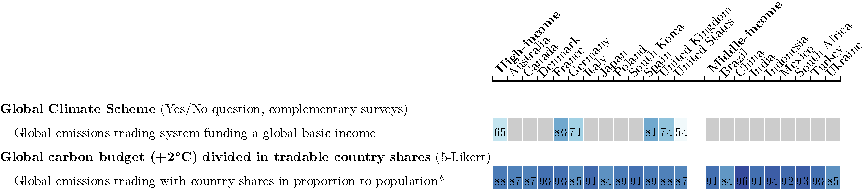
\includegraphics[width=1.2\textwidth]{../figures/OECD/Heatplot_global_tax_attitudes_only_GCS_share.pdf}} 
    % \makebox[\textwidth][c]{\includegraphics[width=1.2\textwidth]{../figures/OECD/Heatplot_global_tax_attitudes_GCP_share.pdf}} 
\end{figure}

To assess the robustness of the public support found in the 20 countries, \citet{fabre_international_2023} run complementary surveys on 3,000 U.S. respondents and 3,000 European ones (in France, Germany, Spain, and the UK). They describe the GCP as in Section \ref{sec:intro}, detailing the negative effects on the respondents' purchasing power. Despite its costs being made salient, the GCP still obtains majority support of 54\% in the U.S. and 76\% in Europe. Using a technique called list experiment, they further show that the support is genuine and not driven by a potential social desirability bias. Actually, a majority of people in each country is willing to sign a petition in favor of the GCP, knowing that the share of respondents willing to sign will be transmitted to the head of State's office. 

The most compelling evidence showing that the support for the GCP is profound, is that a progressive candidate may win voting shares by endorsing it. \citet{fabre_international_2023} show this using different questions. First, they present a progressive and a conservative platform, frame the choice as the next election, and ask respondents which candidate they would vote for. Adding the GCP to the progressive platform for a random half of the sample, they show that, in France, the progressive candidate would win 11 points by endorsing the GCP. In the U.S., the progressive candidate could win 3 points (the $p$-value is .13) while in the other countries, the effect is not significantly different from zero (even at the 20\% threshold). Second, they draw two political platforms at random from a pool of (rather progressive) policies, and then add the GCP to one of the platform. In Europe, respondents are prompted to imagine that a left- or center-left coalition will win the next election and are asked what platform they would prefer that coalition to have campaigned on. In the U.S., the question is framed as a hypothetical duel in a Democratic primary, and asked only to non-Republicans. The platform containing the GCP is preferred by a majority (from 58\% in the U.S. and the UK to 64\% in Spain). Finally, using a question asking respondents to allocate 100 points to express their support to different policies, \citet{fabre_international_2023} show that the GCP is more prioritized than the average policy and is among the most preferred climate policies, while a policy enacted in the EU and California (the phase out of new combustion-engine cars) is one of the three least prioritized policies in each country. 


\section{Details of the plan}\label{sec:details}

Some points remain to fully specify the GCP: its timeline, scope, framework, governance, market design, and participation mechanisms. 

\paragraph{Timeline} 
The GCP can be put at the agenda in the UNFCCC and the G20, aiming at a gradual phase-in between 2030 and 2035. During the negotiation and preparatory phase (before 2030), it is crucial to ask people around the world whether they would like to receive a basic income and survey their potential concerns. Indeed, each community should have the right to opt out of the basic income (or receive it in a different form, for example as a transfer to the community as a whole rather than to individuals), to avoid disrupting social structures. Furthermore, the basic income should begin with very low amounts to make sure that its delivery runs smoothly. Indeed, the redistribution operated by the basic income would lead to an increased demand for (and a higher price of) basic commodities. Despite the inflation, the basic income would increase low-income people's purchasing power, but it is important to leave no one behind and make sure that everyone who wants the basic income receives it. % If the ETS is ready before the basic income, it could be implemented with each country retaining most of the revenues it collects

\paragraph{Scope} 
The GCP would regulate exclusively CO$_\text{2}$ emissions. Although similar policies can be designed to regulate other substances, it is more suited to treat the CO$_\text{2}$ separetely to better handle its specificities. Ideally, the GCP would cover all CO$_\text{2}$ emissions, though it may be more practical to initially limit it to CO$_\text{2}$ from fossil fuels and cement production in large industrial units (i.e. the same scope than the EU ETS and ETS2 combined). The GCP should also cover CO$_\text{2}$ emissions from international shipping and aviation. 

\paragraph{Framework} 
The international treaty instituting the GCP should specify some non-modifiable elements, including its scope, the use of its revenues, its rules of governance, and the carbon budget. The carbon budget should be defined by an interpretation of the Paris agreement's objective of 
``Holding the increase in the global average temperature to well below 2 \textdegree{}C above pre-industrial levels and to pursue efforts to limit the temperature increase to 1.5 \textdegree{}C above pre-industrial levels''. A possible interpretation is that we aim for a long-term temperature of +1.5\textdegree{}C but allow an overshoot up to +2\textdegree{}C. 
This would define a carbon budget of 500 GtCO$_\text{2}$ starting in 2020 \citep{ipcc_climate_2021}, translating into the GCP's carbon budget by subtracting emissions occurring between 2020 and the launch of the GCP. The full trajectory, including the negative emissions allowed,\footnote{Carbon (positive) emissions could exceed the carbon budget by the amount of negative emissions allowed, as the negative emissions would eventually absorb the excess CO$_\text{2}$.} could then be chosen in accordance with the maximum overshoot target and up-to-date understanding of the climate system. A more flexible interpretation might be used if we consider a stricter target unattainable (given the current emissions of 41 GtCO$_\text{2}$ per year). Alternative interpretations could be limiting global warming to +2\textdegree{}C with 83\% probability (entailing a budget of 900 GtCO$_\text{2}$ from 2020) or with 67\% probability (1150 GtCO$_\text{2}$). % TODO find how many in our GEA scenario

If some countries do not participate in the GCP, the GCP's carbon budget would be adjusted downward on the basis of an equal right to emit for each human adult (consistent with leaving the same rights to emit to non-participating countries).

\paragraph{Governance} 
The governing body of the GCP would define the yearly emissions quota (in line with the GCP framework), the market design, and possible sanctions against non-participating countries. The choice of sanctions would be the most political decision of the body. It would mostly affect powerful countries, as they are the main geopolitical actors, therefore those that the sanctioned countries might target in possible retaliations. Moreover, the ETS would directly affect participating countries according to their emissions. It thus seems legitimate to grant each country a voting right proportional to its carbon emissions, at least for decisions pertaining to the ETS or sanctions. For decisions relative to the basic income, each country would have a voting right proportional to its adult population. 

When the body has to choose between several options, it should use approval voting, and when these options are numeric, use the median preferred value. Finally, each country should be allowed to have multiple representatives, to choose how its representatives are appointed (possibly through elections) and how the country's voting rights are split among these representatives. 

\paragraph{Market design} 
The compliance period to surrender emissions permits should be one calendar year, and the quota should be adjusted each year. Carbon offsets should not be allowed as a substitute to surrender emissions permits. Borrowing and banking emissions permits should be limited in time and quantity to avoid speculation. % Borrowing emissions permits should be forbidden and banking should be limited in time and quantity to avoid speculation. 

\paragraph{Participation mechanisms}

The basic participation mechanism, which would also prevent carbon leakage, is a carbon border adjustment: non-participating countries would face a tariff on the goods they export to participating countries according to the emissions embodied in these goods (or according to a worst-case benchmark if these emissions cannot be measured). The carbon price applied to such exports would be at least equal to the market price. The governing body could decide to apply a higher price, on two grounds. First, if non-participating countries (with higher-than-average carbon footprint) joined the GCP, the GCP's carbon budget would grow less than the set of regulated emissions, so the market price of carbon would rise. The carbon price should be equal to that higher level (all over the world) to respect the carbon budget. Therefore, the carbon border adjustment could be set at (the estimated value) of that \textit{counterfactual price}, to internalize the price that participating entities would have to pay for these imported goods if the GCP was truly global and the carbon budget respected. Second, the governing body could decide to apply sanctions in the form of a tariff higher than the counterfactual price. 

In some federal countries like the U.S., some States may be willing to join the GCP while the federal level would not. The GCP would add provisions to help such States to join it. In particular, participating subnational entities would be allowed to opt out from levying a carbon border adjustment, and they may choose % would also be allowed 
to use their allocated revenues differently than by delivering a basic income. 
In this way, a State like California could use GCP revenues to subsidize manufacturing firms, perpetuating its way of recycling ETS revenues and preventing carbon leakage while being part of a national customs union. % 10322/25463 of U.S. 2022 GDP in States with +15% margin for Democrats.

\begin{figure}[b!]
  \caption{Net Present Value of the Global Climate Plan by country.}\label{fig:median_gain_adj}
  \makebox[\textwidth][c]{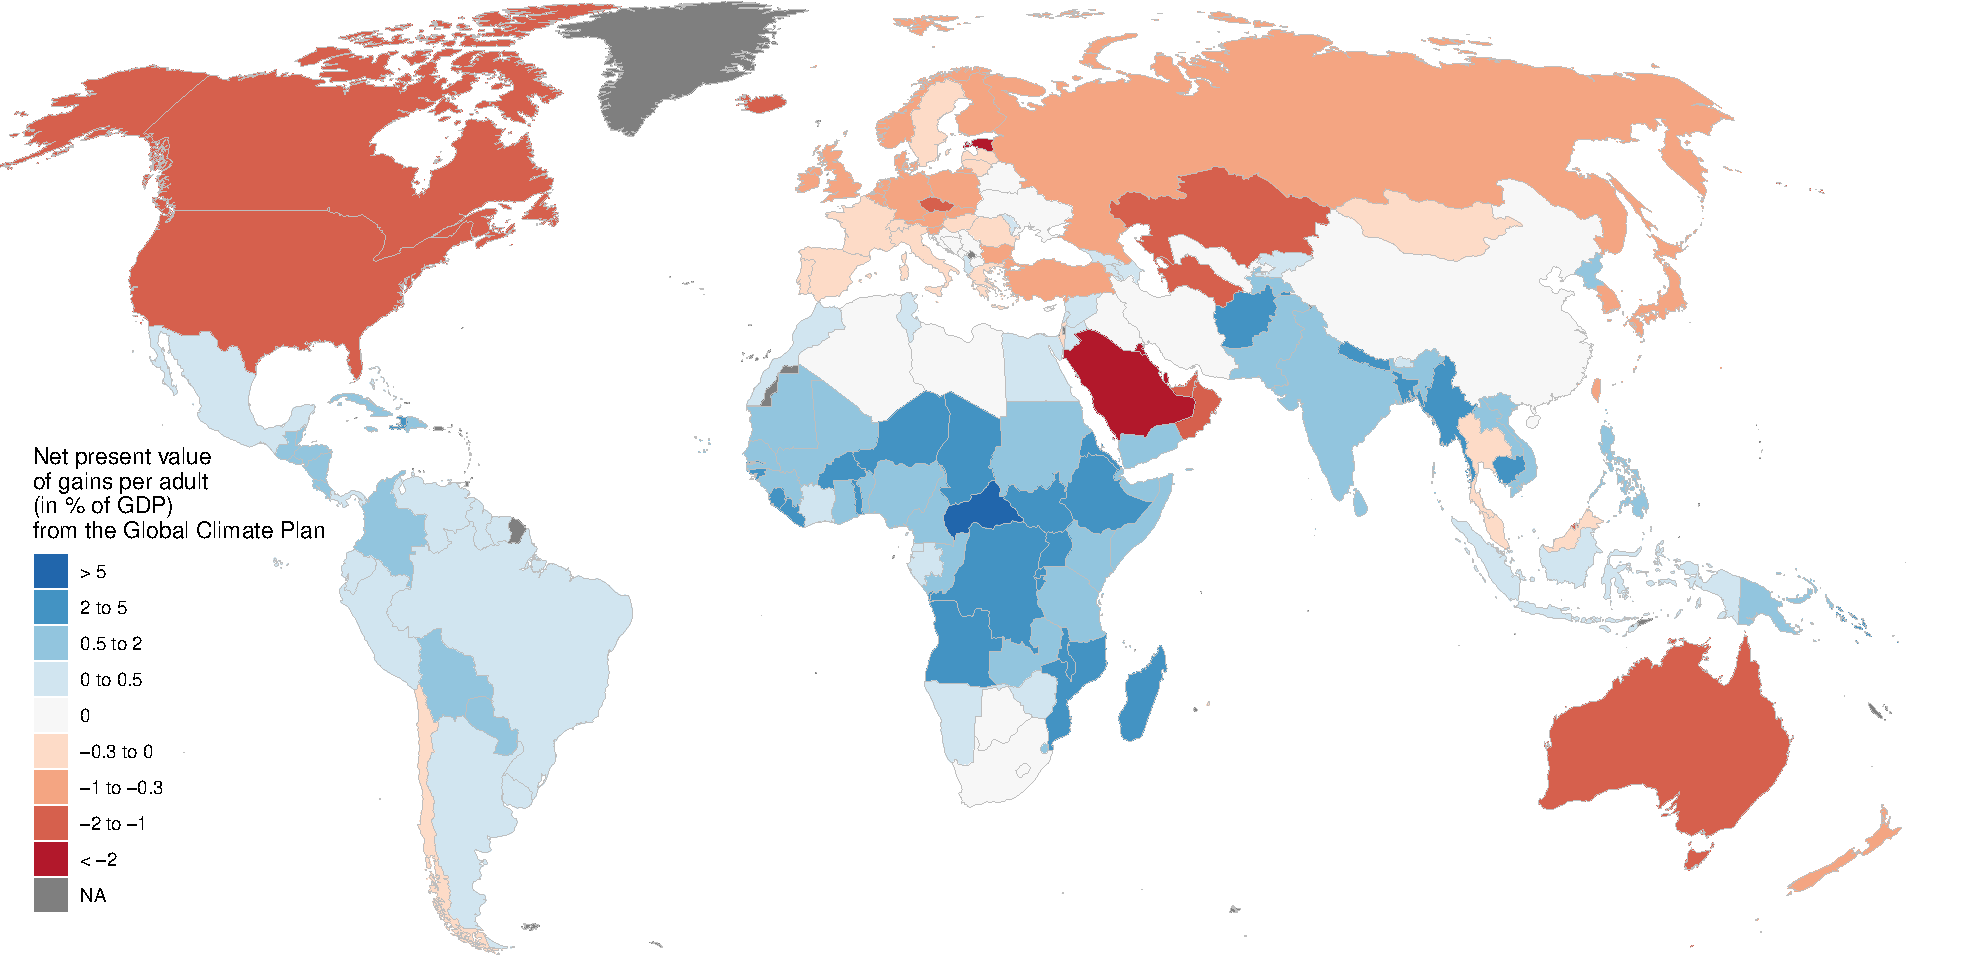
\includegraphics[width=\textwidth]{../figures/maps/npv_over_gdp_gcs_adj.pdf}} % mean_gain_over_gdp_2019
  {\footnotesize \textit{Note:} The Net Present Value is computed with a 4\% discount rate over the period 2020 -- 2100.}
\end{figure}

Although high-income countries have the ability and the duty to help low-income countries decarbonizing and alleviating global poverty, this responsibility does not seem to apply to countries around the world average income per capita (\textit{intermediary countries} for short). Yet, some intermediary countries like China have a higher-than-average carbon footprint. To encourage such countries to participate in the GCP, we could allow them to opt out from the mutualization of revenues and the basic income, under certain conditions. To be authorized to fully opt-out and retain the auction revenues collected on its territory, a country should have a GNI per capita below 1.5 times 
the world average (in nominal terms).\footnote{Currently, the world average is at \$13,200 per year while China is at 11,900 and Russia at 11,600.} Countries richer than this threshold % the average
would be eligible to a partial opt-out, to the extent that their GNI p.c. is below twice the world average. For example, a country with a GNI p.c. 70\% above the average would have to mutualize 40\% of the revenues from its territorial emissions, but could retain 60\% of these revenues, in which case it would receive only 40\% of the basic income. Mutualization opt-outs would reduce the basic income from \$56 to \$47 per month in 2030 in countries that do not opt out. 
A potential concern with this participation mechanism is that it would give too large an advantage to large exporters, i.e. opting-out countries with territorial emissions substantially larger than their carbon footprint. Indeed, these countries would retain revenues corresponding to their net exports of carbon emissions, making the basic income lower than the average increase in individual expenditures (for countries that do not opt out). However, note that the carbon border adjustment enacted by the EU gives the exact same advantage to foreign exporter countries with an internal carbon price equal to the EU-ETS price: imports from these countries would be exempted from the carbon border adjustment, and these countries would benefit from carbon price revenues eventually paid by European consumers. Still, we can limit the opt-out advantage, for example by establishing a limit on the revenues that can be retained, e.g. at 50\% above the average global revenues per adult. % TODO implement
Besides, the advantage to opt-out could be granted in exchange for some condition, such as the participation to a global wealth tax with a share of the revenues pooled to finance low-income countries. %The share of the global wealth tax not retained by the collecting country can be computed to offset the advantage due to collecting GCP revenues in function of territorial emissions rather than the carbon footprint. Doing so could discourage opting-out countries to leave the GCP and set an internal carbon price equal to the GCP (effectively reproducing the opt-out situation outside the GCP). Indeed, the governing body could impose to these countries a carbon border adjustment at the counterfactual price, making them in principle indifferent between participating in the GCP and transferring resources through the wealth tax, or not participating and paying the carbon border adjustment. % => wrong, because CBA incidence falls on consumers, i.e. importers


Conversely, some high-income countries might have a lower-than-average carbon footprint in the future, especially in 1.5\textdegree{}C-trajectories (this would occur around 2050 in the SSP1-1.9 scenario of \citealp{van_vuuren_energy_2017}). To prevent the GCP from entailing transfers from higher income to lower income countries, a provision could specify that high-income countries cannot receive the basic income if their emissions per adult are lower than the global average. To avoid threshold effects, the basic income received by a country with a GNI p.c. above 2 times the world average ($\overline{y}$) and territorial emissions p.c. below 1.3 times the average of (non opting-out) participating countries ($\overline{e}$) could be a function of these two variables, defined in such a way that a carbon-neutral country 2.2 times above the GNI p.c. average would no longer received the basic income. Denoting $y$ a country's GNI p.c., $e$ its emissions p.c., and $B$ the unadjusted basic income (i.e. total revenues divided by population of participating countries), if $2\overline{y}\leq y\leq 2.2\overline{y}$ and $e \leq 1.3 \overline{e}$, the basic income for that country would be $\left( \frac{2.2\overline{y}-y}{0.2\overline{y}} + \frac{e}{1.3\overline{e}} \frac{y-2\overline{y}}{0.2\overline{y}} \right) B$. The basic income (in countries not concerned by this provision) is then adjusted upwards using the freed revenues.

% alternatives: other particpation mechanisms, etc: 
% G est intégré (A, sa version idéale à partir d'empreinte carbone, est écarté faute de données), E est intégré (B, sa version extrême, est écartée), F est en TO-DO ailleurs, C et D (prenant en compte plus (C) ou moins (D) les respos historiques) sont intéressants mais écartés (pour ne pas se disperser)

% Pistes pour éviter des transferts des pays pauvres vers les riches et que la Chine ne perde trop:
% $>$ A. Que les pays à moyens (ou bas) revenus puissent se retirer (opt out) de la mutualisation des recettes et du revenu de base. La banque mondiale définit le seuil de hauts revenus à un GNI pc nominal de 13.2k (Chine: 11.9, Russie: 11.6, Arabie Saoudite: 21.5k, monde: 12k). On pourrait aussi choisir un seuil plus élevé (e.g. deux fois le GNI pc mondial soit 24k).
% Pb: Sortir de la mutualisation casse la logique, difficile de calculer l'empreinte carbone. Effet de seuil. 

% $>$ G. Comme ci-dessus mais pour les pays s'étant retirés, on calcule leurs recettes sur la base des émissions territoriales (avec une borne max à +50\% des émissions mondiales moyennes). Et on ne les autorise à se retirer que s'ils participent à la taxation des millionaires en partie redistribuée aux pays pauvres. On calcule la taxe sur la fortune de sorte que ça compense le gain qu'ils obtiennent les recettes en fonction de leurs émissions territoriales plutôt que de leur empreinte. S'ils refusent la taxation des millionaires (et donc l'accord) et mettent en place une tarification des émissions unilatérale du même montant que dans l'accord, on met quand même en place un CBAM. En effet, on calcule le quota des pays de l'accord sur la base d'un égal droit à polluer pour chaque humain, ce qui laisse au pays hors accord exportateur d'émissions un droit à polluer inférieur à ses émissions. Comme le prix du carbon serait supérieur s'il rejoignait l'accord, on taxe ses émissions davantage. 
% =$>$ calculer le montant nécessaire -$>$ Environ .1\% du PIB mondial pour la Chine (cf. policy\_brief\_tax). Si 1/3 est reversé aux paus à bas revenus, il faut une taxe qui rapporte .3\% du PIB mondial en Chine, soit $\approx 2\%$ du PIB mondial en tout. Ce qui est faisable en ne s'attaquant qu'aux fortunes $>$5M et sans même les réduire (taux max de 7\%). Ça opérerait un transfert de $\approx.6\%$ du PIB mondial, du même ordre que le $\approx$.75\% du GCP. À comparer au .85T\$ (surestimé, cf. calcul dans map\_GCP\_incidence.R) nécessaire pour résorber le poverty gap à 3.65\$ (il est de 4T pour le pg à 6.85\$/day) % TODO! faire ces calculs dans le position paper (ou en off)
% =$>$ Pb: Effet de seuil + ça opèrerait un transfert des pays importateurs de la Chine à la Chine, puisque la Chine récupèrerait les recettes des émissions territoriales liées à ses exportations. Certes, mais c'est déjà comme ça que sont envisagés les fusions de marchés carbone ou CBAM (article 9), et le transfert ne serait pas énorme puisque les importateurs ne touchent qu'une part d'entre elles correspondant à leur population (les autres perdants seraient les pays à bas revenus qui verraient leur revenu de base diminué). Pour éviter l'effet de seuil, on peut dire que si le GNI pc du pays relatif au GNI pc mondial est de $1+y\in [1;2]$ alors une fraction y est mise en commun.

% B. Les pays à hauts revenus renonceraient aux recettes. Ça augmenterait le revenu de base de \~20\%, et diviserait par près de deux la perte de la Chine.
% Pb: Pas sûr que les pays riches acceptent. Pas sûr que ça suffise pour convaincre la Chine.

% C. Compléter la mesure par l'établissement d'une dette carbone due aux responsabilités historiques (entre 1990 et l'entrée en vigueur de l'accord). Le financement des émissions négatives devra être assuré au pro rata des dettes carbone.
% Pb: Difficile de calculer l'empreinte carbone et de choisir une convention sur la population. Rompt avec la logique de taxer les individus. Pas sûr que la Chine accepte de payer en échange d'une promesse de transferts (non monétaire mais carbone) futurs. 

% D. Les pays ayant excédé leur budget carbone 1.5°C ne toucheraient pas le revenu de base.
% =$>$ check lesquels c'est
% =$>$ Pb: ça pourrait ptet résoudre le pb que les indiens émettraient plus que les Européens en 2050, mais ne résoudrait pas le pb de la Chine à court terme.

% $>$ E. Si un pays est dans le top 30\% du PIB pc mais en-dessous de la moyenne pour les émissions pc, alors il ne peut pas toucher le revenu de base, et cet argent est à la place reversé aux pays pauvres qui ont des émissions supérieures à la moyenne.
% Pb: Effet de seuil. Sort de la logique du pollueur-payeur (en pratique, réduit le prix global des émissions pour les pays pauvresp polluants). Pas sûr que ça suffise à convaincre la Chine.

% F. Compléter par une taxe sur les millionaires reversée aux pays à moyen et bas revenus du club (ou sous 2*GNIpc moyen), de façon dégressive de leur GNIpc. 
% =$>$ calculer quelle somme doit être versée pour compenser la Chine -$>$ 0.1\% du PIB mondial (leur empreinte est +50\% de la moyenne, et à \~24\% du total, donc les recettes à compenser sont \~6\% du total, qui est 1.7\% du PIB mondial)
% Pb: Les US n'accepteront peut-être pas de tels transferts vers la Chine.

\paragraph{Sanctions}

If the governance body finds it appropriate to encourage participation, it could vote sanctions against non-participating countries, such as tariffs (beyond the carbon border adjustment), assets forfeiture, or travel restrictions (especially targeting elites). 

% TODO:
% - What to do with countries that do not properly allocate the basic income (e.g. do it through tax credit, which doesn't reach poor people - who pay no tax)? 
% => We need to think about this. Sanctions? Like lower basic income for these countries? Idk.
% I suggested that historical responsibilities be taken into account by computing the carbon debt/credit of each country until the GCP kicks in. Climate debt would be repaid through carbon removal. 
% - Warned that climate activists hate carbon removal, so it's better strategically to not mention it.
% - What do creditor countries get in this system? [I don't know, nothing I guess?]
% => Better to say that we tackle historical responsibilities with the global wealth tax and not mention the other thing.

\paragraph{Negotiations}

We tried to be as specific as possible to anchor discussions on a concrete plan that we deem fair. Still, some elements of the GCP can be modified without fundamentally altering it, such as the opt-out threshold or using a tax rather than an ETS. % TODO? explain the difference quota/tax, and mention it before
It is now up to the public and policy makers to take up this proposal and negotiate it. 
\quad \\ \quad 

\textit{We are here to feed the public debate on global redistribution. We welcome counter-proposals, criticisms and suggestions concerning our policy brief (including pull requests). Feel free to engage the discussion on \href{https://github.com/bixiou/global_tax_attitudes/issues}{github}. }

{\footnotesize
\begingroup
\setstretch{.5}
\titleformat*{\section}{\fontsize{11pt}{14pt}\bfseries\selectfont}
\renewcommand{\url}[1]{\href{#1}{Link}} % NCCcomment
\bibliographystyle{plainnaturl_clean} % NCCcomment
\bibliography{global_tax_attitudes}
\endgroup }


\end{document}